
\newpage 
%\chapter{Imperative programming versus declarative programming} 
\chapter{Sum of series. Imperative versus declarative}   \label{chap:impdec}


\section{Introduction}
\vspace{-0.5cm}
A big number of programming languages exist nowadays, all of them covering different features 
in order to fit diverse needs. While a programming languages is focused on the way the 
code is organized, other language gives importance to the dataflow through operations.
Consider as an example the object-oriented paradigm, one of his main features 
is that the data is organized into objects 
that are modified by methods also specified in the object.

%According to these features, the different programming paradigms appear. 
A group of these features define the conceptual framework of the language, its programming paradigm.
Think of it as a group of ideas that describe how to write a program. Some languages are based only on one 
paradigm while others are multi-paradigm so their programs are too.  

A big amount of programming paradigms are commonly grouped into two types: imperative and declarative. 
This chapter covers the difference between both supported on examples of numerical sum series.

In an imperative style, the programmer tells the machine \textbf{how} to perform each task step by step,
hence, an statement describes how to change the state of the program.
However, in a declarative paradigm, the programmer tells the interpreter/compiler \textbf{what} to obtain
and its properties but not the control flow of the process. 



\section{Sum of numerical series} 
One of the main tasks of numerical calculus is to sum numerical series
which appear from approximation of functions to numerical integration. 

The algorithm to sum these series can be done in an iterative way by a sequential machine or von Neumann
machine or concurrently by a bunch of processors.
This first idea allows to introduce the two different paradigms mentioned when trying to write or to implement 
algorithms in different programming languages: imperative paradigm and declarative paradigm. 

Imperative programming is related to an ordered sequence of sentences that allows to obtain the solution
whereas declarative programming is concerned with the specification or the statement of the problem 
no matter the way it is accomplished. 

The following sum series are treated in the Fortran project included with this book:

$$
S = \sum_{n=1} ^{\infty} \frac{ (-1)^{n+1} } { 2^n },  \ \   \ \
S = \sum_{n=1} ^{\infty} \frac{ 1 } { n! },  \ \   \ \
S = \sum_{n=1} ^{\infty} \frac{ 1 } { n^2 }
$$

The first two examples have a good convergence, this means that the general
term $a_n$ tends to zero quickly with  $n \rightarrow \infty$ and few terms must be added 
to get a correct result. 
Then, it is easy to obtain the result of the infinite sum up to a given finite number of digits. 
However, the third example has a poor convergence and some issues must be review to sum it 
in a correct way. The following chapter is dedicated to this third example and the particularities 
that appear when bad convergence series are calculated with a finite precision machine. 


%--------------------------------------------------------------------------------------------
%--------------------------------------------------------------------------------------------
\newpage 
\section{First example with imperative paradigm} 
Let's consider the following summation  as an example to show how the imperative paradigm 
can be implemented. 
$$
S_N = \sum_{n=1} ^{N} \frac{ 1 } { n^2 }
$$
In the following code, the summation is done in an iterative way. 
\vspace{0.5cm}
\renewcommand{\home}{./Fortran/sources/Foundations/Calculus} 
\listings{\home/Examples/Sum_series.f90}{function SummationN_n2}
          {end function}{Sum_series.f90}
          

The result for \texttt{N = 10} is obtained by calling the function in the following way:
\begin{verbatim} 
    write(*,*) " S = ", SummationN_n2( 10 ) 
\end{verbatim}

Notice how the main task to develop (sum a value to the older value of \texttt{S}) is specified to the 
compiler with a loop. Since this function is simple, the imperative style used is easy to read and easy to 
learn for beginners. However, with more complex tasks, the code quickly becomes extensive and difficult 
to follow and maintain.

If you are curious about the need of including \texttt{real(i)} in the denominator of the sum, 
this issue is treated in the section \ref{sec:NumIssues} and also you can take a look 
at the chapter \ref{sec:UndersIntOver}. Just forcing the number \texttt{1.} of the numerator to be real, 
the operations are performed in the reals field so the result is properly calculated, converting the denominator to 
real should not be needed. However, there is another interest in doing that. As a clue, overflow of integers must be avoided. 
    
    
\newpage 
\subsection*{Python code} 
This example can be implemented with Python in a similar way.
Notice that data type for variables (\texttt{S}, \texttt{i} or \texttt{N}) is not explicitly declared, 
Python automatically declares it when a value is assigned. Also, indentation rules are strictly followed and 
there is no need to close structures like loops by means of statements. 
\vspace{0.5cm}
\renewcommand{\home}{./Python/sources/Foundations/Calculus} 
\lstpython
\listingsp{\home/Examples/Sum_series.py}{def SummationN_n2}
          {return}{Sum_series.py}          
\lstfor


\newpage 
\section{First example with declarative paradigm}
Now the same sum is coded with declarative programming. On one hand, the abstraction of 
summation is used for the function \texttt{Sigma\_N}, an easily reusable code has been created and once 
validated it will be used for future similar projects. On the other hand, the general term of the sum 
is independently declared in a different function, hence, if the program specifications change 
(a different sum is needed), updating this code is extremely easy. 

\vspace{0.5cm}
\renewcommand{\home}{./Fortran/sources/Foundations/Calculus} 
\listings{\home/Series.f90}{function Sigma_N}
          {end function}{Series.f90}

\vspace{0.5cm}
\renewcommand{\home}{./Fortran/sources/Foundations/Calculus} 
\listings{\home/Series.f90}{interface}
          {end interface}{Series.f90}

\vspace{0.5cm}
\renewcommand{\home}{./Fortran/sources/Foundations/Calculus} 
\listings{\home/Examples/Sum_series.f90}{function a1}
          {end function}{Sum_series.f90}



The result for \texttt{N = 10} is obtained by calling the function in the following way:
\begin{verbatim} 
    write(*,*) " S = ", Sigma_N( a1, 1, 10 ) 
\end{verbatim}

\newpage
The essence of the declarative programming in this example are the lines:

\texttt{S = sum( [ (a(i), i=i0, N ) ] )} 
 
\texttt{Sigma\_N( a1, 1, 10 )}

Both lines tell the compiler the properties of the solution to be obtained, no matter how the process is done. 
In the first case the intrinsic function \texttt{sum} performs the summation 
of the elements of a Fortran vector by means of an implicit loop from one value to another. The properties of the solution sought are 
of course the limits of the sum (\texttt{i0} and \texttt{N}) and the type of term to be added. 
In the second case, thanks to the created function \texttt{Sigma\_N}, the sum is performed just by declaring the 
general term to add and the limits, the programmer does not need to tell the compiler how to do the summation step by step.

Another ingredient is needed for this example, since the function \texttt{Sigma\_N} admits any general term 
of a series, it needs to know how to communicate with the function that defines that general term \texttt{a1(n)}. 
Through the interface block (intentionally created defining a function from integers to reals) \texttt{Sigma\_N}
knows everything about the dummy arguments used inside the referenced procedure \texttt{a1(n)}. The same procedure 
could be recycled next time a function of the following form is used: 
$$ 
\myfunc{ \texttt{f\_N\_R} }{\mathbb{Z}}{\mathbb{R}}{n}{\texttt{f\_N\_R(n)}} 
$$
\subsection*{Python code}
The same advantages demonstrated with Fortran are visible in Python, 
now the extension and simplicity of the code is even higher due to the characteristics of this language. 
We do not need vectors in Python since lists, the representation of matheamtical sequences, are built-in in the language. 
However, do not forget the implicit assumptions that are made for its statements; 
type and kind of variables, interface between procedures, etc.  
\vspace{0.3cm}
\renewcommand{\home}{./Python/sources/Foundations/Calculus} 
\lstpython
\listingsp{\home/Series.py}{def Sigma_N}
          {return}{Series.py}  
\vspace{0.2cm}
\listingsp{\home/Examples/Sum_series.py}{def a1}
          {return}{Sum_series.py}



%--------------------------------------------------------------------------------------------
%--------------------------------------------------------------------------------------------

\newpage 
\section{Second example with imperative paradigm} 
Let's consider another series summation example with imperative paradigm. 
In this case the result sought is the summation of the infinite terms of the series. 
$$
S = \sum_{n=1} ^{\infty} \frac{ 1 } { n^2 }
$$
In the following code, the summation is done in an iterative way. 
\vspace{0.5cm}
\renewcommand{\home}{./Fortran/sources/Foundations/Calculus} 
\listings{\home/Examples/Sum_series.f90}{function Summation_n2}
          {end function}{Sum_series.f90}

This piece of code performs the summation of as many terms as 
the variable \texttt{S} can significantly sum to itself. 
Once the nth term of the sum is not going 
to modify the value of \texttt{S} due to its finite number of digits, 
the result obtained is the closest value
to the infinite sum that \texttt{S} can hold (with this specific algorithm). 
Then, \texttt{n} is returned indicating the last term calculated. 

The sum must be stopped once the result of \texttt{an} is smaller than the 
smallest number that can be added to \texttt{S}. Then, the result of 
adding \texttt{S + an} is equal to \texttt{S}. Notice that the calculus of \texttt{S}
from one step to the next one is the same to the first example. However, now \texttt{Sn}
is used to compare the value before and after the nth sum. If both values are the same, 
it means that \texttt{an} has not contributed to \texttt{S} and the process is stopped. Also, 
take into account the need of
initializing \texttt{S} and \texttt{Sn} with different values.
 
\newpage
The result of the sum is obtained by calling the function in the following way:
\begin{verbatim} 
    integer :: n
    
    write(*,*) " S = ", Summation_n2( n )
\end{verbatim}


\vspace{0.5cm}

\subsection*{Python code}
The same imperative statements are presented now with Python.  

\vspace{0.5cm}
\renewcommand{\home}{./Python/sources/Foundations/Calculus} 
\lstpython
\listingsp{\home/Examples/Sum_series.py}{modify arguments}
          {return S}{Sum_series.py}
\lstfor





\newpage
\section{Second example with declarative paradigm}  \label{sec:Sigma}
For this example a modification of \texttt{Sigma\_N} is needed: \texttt{Sigma}. Nevertheless, notice the simplicity of the code when 
the existing function \texttt{Sigma\_N} is reused.

For an infinite sum it is more interesting to declare the minimum term to add to the sum (\texttt{eps}) instead of the number of 
terms to sum (\texttt{N}). The programmer does not normally know how many terms are needed to reach a finite number of digits in the result.
However, the allowed error of the result is usually a specification. 
%the minimum term that his result can store in order to calculate it. 
For this reason, \texttt{N} is automatically found by specifying the general term and the 
minimum term to sum with the function \texttt{Tail(a, eps)}. 
Then, \texttt{Sigma\_N} is used to perform the sum as seen in the previous example. 

Once again, the operation is performed by means of a desired properties bunch and not declaring the control flow step by step. 
This strategy increases the capabilities of solving many different problems with the same tools by creating more and more complex functions 
always based on lower level functions (in a hierarchical structure). In this case for example, a new degree of freedom (\texttt{eps}) 
is obtained by using \texttt{Sigma}, which is based on \texttt{Tail} and \texttt{Sigma\_N}. 
This programming paradigm also leads to a reuse strategy, where the next time that a similar task is performed 
in another program, the same functions can be used thereby saving time.


\vspace{0.5cm}
\renewcommand{\home}{./Fortran/sources/Foundations/Calculus} 
\listings{\home/Series.f90}{function Sigma}
          {end function}{Series.f90}

\newpage 
\vspace{0.5cm}
\renewcommand{\home}{./Fortran/sources/Foundations/Calculus} 
\listings{\home/Series.f90}{function Tail}
          {end function}{Series.f90}

Do not forget to declare the same interface block of the first example \texttt{f\_N\_R(x)} and define 
the general term to sum (\texttt{a1} for example), then, the following statements obtain the infinite sum
for a minimum general term of \texttt{eps = 1e-10}:
\begin{verbatim} 
    real :: eps
    
    eps = 1e-10
    write(*,*) " S = ", Sigma( a1, 1, eps ) 
\end{verbatim}




The mathematical support for the function \texttt{Tail} is treated in the section \ref{sec:NumIssues}. 
It is essential to notice three issues:

\begin{enumerate}
    \item This function is written for good convergence series since its definition is based on 
    obtaining \texttt{N} such as the integral from \texttt{i = N+1} to infinity of \texttt{a\_i} is equal to \texttt{eps}. 
    Read the following section for more information.
    
    \item The stop condition is established on the last two terms to be added with the line:
    
    \texttt{abs( a(i) + a(i+1) ) > 2*eps}
    
    This is done so alternating sums also reacts to this criteria. 
    If this were not done, an alternating sum with very different odd and even terms could stop 
    prematurely.
    
    \item Also, a maximum allowed sums are permitted with the line:
    
    \texttt{.and. i < Nmax} 
\end{enumerate}





\newpage 
\subsection*{Python code}
The same reused strategy is performed with Python by creating the corresponding function \texttt{Tail} and using \texttt{Sigma\_N}.
\vspace{0.5cm}
\renewcommand{\home}{./Python/sources/Foundations/Calculus} 
\lstpython
\listingsp{\home/Series.py}{def Sigma}
          {return}{Series.py}
\lstfor

\vspace{0.5cm}
\renewcommand{\home}{./Python/sources/Foundations/Calculus} 
\lstpython
\listingsp{\home/Series.py}{def Tail}
          {return}{Series.py}
\lstfor





\newpage 

\section{Numerical issues} \label{sec:NumIssues} 
 
    \subsection{Theoretical framework}
From the numerical point of view, there are some important issues to revise.  
Let's try to explain these issues with an example. 
Consider the previous sum of infinite terms: 
$$
S = \sum_{n=1} ^{\infty} \frac{ 1 } { n^2 }.
$$
The difficulty in this case comes with the infinite number of terms to be added. 
It is clear that the program  will try to yield an 
approximate number for this problem and the difficulty will be associated to those 
series with low convergence rate. 
 

\begin{enumerate} 
  %  \setlength\itemsep{-0.3cm}	
    \item Convergence of the series.
 
 The rate of convergence of this series depends on the velocity the general term
 $ a_n =1/n^2$ tends to zero with $ n \rightarrow \infty $. In this special case, $ n $ should be very big to approach $ a_n $ to zero and 
 many terms of the series should be added to obtain the right result. This issue would slow down the process of the summation. Besides, 
 another issue appears associated to the finite precision of computers.  
    
    
    
    \item Overflows associated with integer variables. 
    	
Another interesting issue that we can encounter when running a loop is overflow of variables. A real variable can hold a huge number and an 
overflow is unlikely reached.  
However, since the maximum of an integer variable of 4 bytes is around $ 2 \times 10^7 $, a simple operation such as $ (100)^5 $ can give 
rise to an overflow if the operation is done with integers. Taken into account that the maximum value of a real variable of 4 bytes is 
around $ 3 \times 10^{38} $ and to avoid this issue, the operation 
$ (100)^5 $  can be done with real numbers. 
This is done in the  summation example by the following line: 

\vspace{0.5cm}
\renewcommand{\home}{./Fortran/sources/Foundations/Calculus} 
\listings{\home/Examples/Sum_series.f90}{real to avoid overflow}
          {overflow}{Sum_Series.f90}    
    
    
    
    \item Round-off errors associated to significant digits. 

Since the numbers in the computer are operated with a finite precision arithmetic, real numbers do have an approximate representation. 
This means that they are approximated by a finite number of digits. Namely, single precision variables are approximated 
with 7 digits and double precision variables with 16 digits. Hence, even real number can be very small, the smallest real number $ \epsilon $ 
that can be added to 1 should be greater $ 10 ^{-15} $. 
It is interesting to bound the error committed due to leaving this infinite number of terms out of the sum. 
This forces to stop the summation process when round-off is encountered as 
it is done by the following line in the summation example: 


    \vspace{0.5cm}
    \renewcommand{\home}{./Fortran/sources/Foundations/Calculus} 
    \listings{\home/Examples/Sum_series.f90}{do while}
            {do while}{Sum_Series.f90}    
  
  
    \item Round-off errors associated to the summation process. 
 
Another source of error appears due to the same fact explained above, the finite precision floating point arithmetic
(each of the sums is performed and stored with a finite number of digits; 7 or 15). 
When only one sum is made, this error remains bounded, however, after millions of operations it can grow. 

The total error of the result can be divided into truncation error $E_N$
and round-off error $ E_{fl} $ as follows: 
$$
     E = E_N + E_{fl}.
$$

Since only $ N $ terms are added, and when considering exact precision arithmetic, 
the error is due to those terms from $ N+1 $ to infinity which are not included.    
However, when floating point precision is considered, round-off errors are
accumulated after a huge amount of operations to yield an additional round-off error $E_{fl}$.
An analytical effort is needed to bound the truncation error $E_N$. 
It is important to discuss the magnitude of those two errors 
to optimize the computational effort associated to $ N$.  




%  the The error due 
%to the round-off associated to significant digits ($E_N$) considers the fact that we are not adding an infinite number 
%of terms after N.
%
% Secondly, each of the sums is also 
%performed with finite digits so an error could be accumulated 
% ($E_{fl}$ for floating point error). 

  
    
	\item Truncation error. 
    
The number of terms $ N $ that the algorithm will sum depends mainly on the 
convergence rate of the general term $ a_n $. To know the error associated to 
the finite sum $ S_N $, the remaining terms should be evaluated.

	$$
	   S = S_N + \sum_{n=N+1} ^{\infty} a_n 
	$$ 

\end{enumerate}



To obtain an upper and lower bound of this error the integral test is used. 
Let's consider 
the real function $ f(x) $  that verifies $ f(n) = a_n $ for all $n$.   
This function is represented in figure \ref{fig:sn}. 
In the same figure, the image of $ f(x) $ for different natural values $ n $  
is plotted. These images allow to draw rectangles of height $ f(n)$ and base one. 
From figure  \ref{fig:sn}, 
the integral from $ n $ to $ n+1 $ can be bounded by the area of two rectangles of height $ f(n+1) $ and $ f(n) $ 
by the following expression:
\begin{equation} 
f(n+1) \le \ \int _{n} ^{n+1}  f(x) \ dx \le \ f(n) 
\label{fnb}
\end{equation} 
Since the  error $ S - S_N $ is given by:  
$$
S-S_N = \sum_{n=N+1} ^\infty f(n)
$$
and using equation (\ref{fnb}), a lower bound for the error is obtained: 
$$
S-S_N \ge \sum_{N+1}  ^\infty \int _{n} ^{n+1}  f(x) \ dx = 
\int _{N+1} ^{\infty}  f(x) \ dx.
$$
In the same manner, an upper bound is given by: 
$$
S-S_N = \sum_{n=N} ^\infty f(n+1) \le \sum_{N}  ^\infty \int _{n} ^{n+1}  f(x) \ dx = 
\int _{N} ^{\infty}  f(x) \ dx
$$
With these bounds, the rest $ S- S_N $ can be estimated by the following expression: 

\begin{equation}
  \int _{N+1} ^{\infty}  f(x) \ dx\  \le \ S -S_N \ \le \int _{N} ^{\infty}  f(x) \ dx
\label{error_SN}
\end{equation} 


\begin{figure}[h]
	\centering
	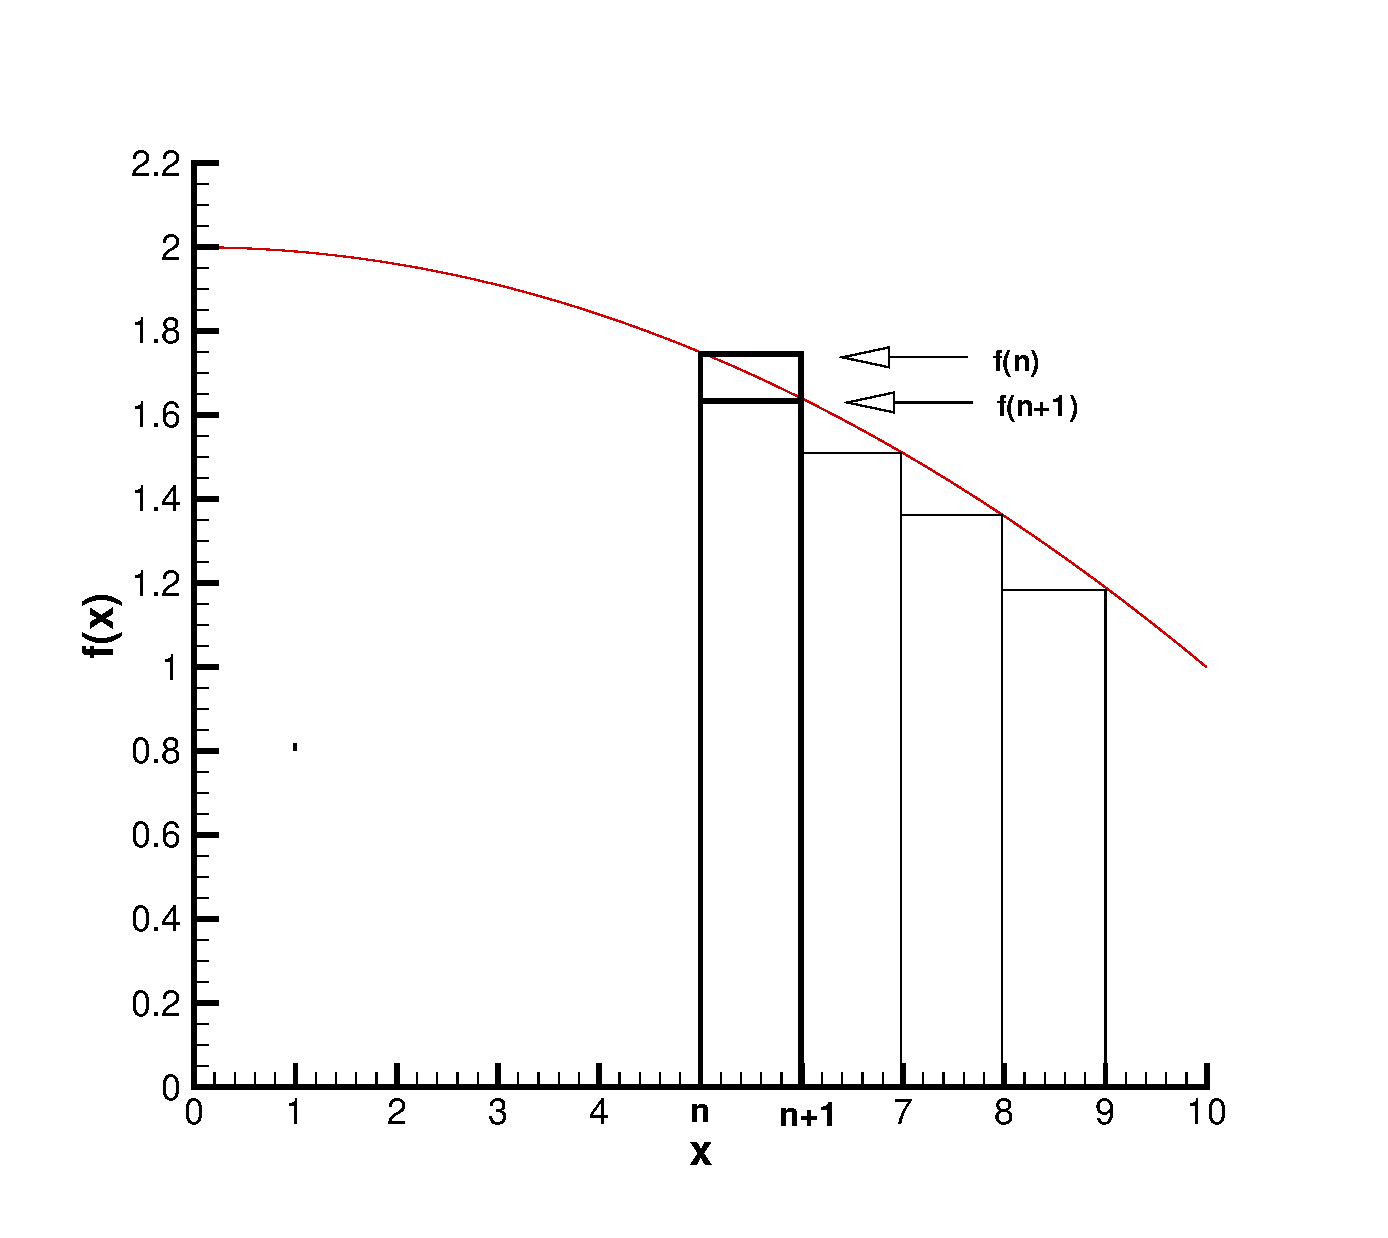
\includegraphics[width= 0.9\textwidth]{./doc/Figures/tecplot/snb}
	%	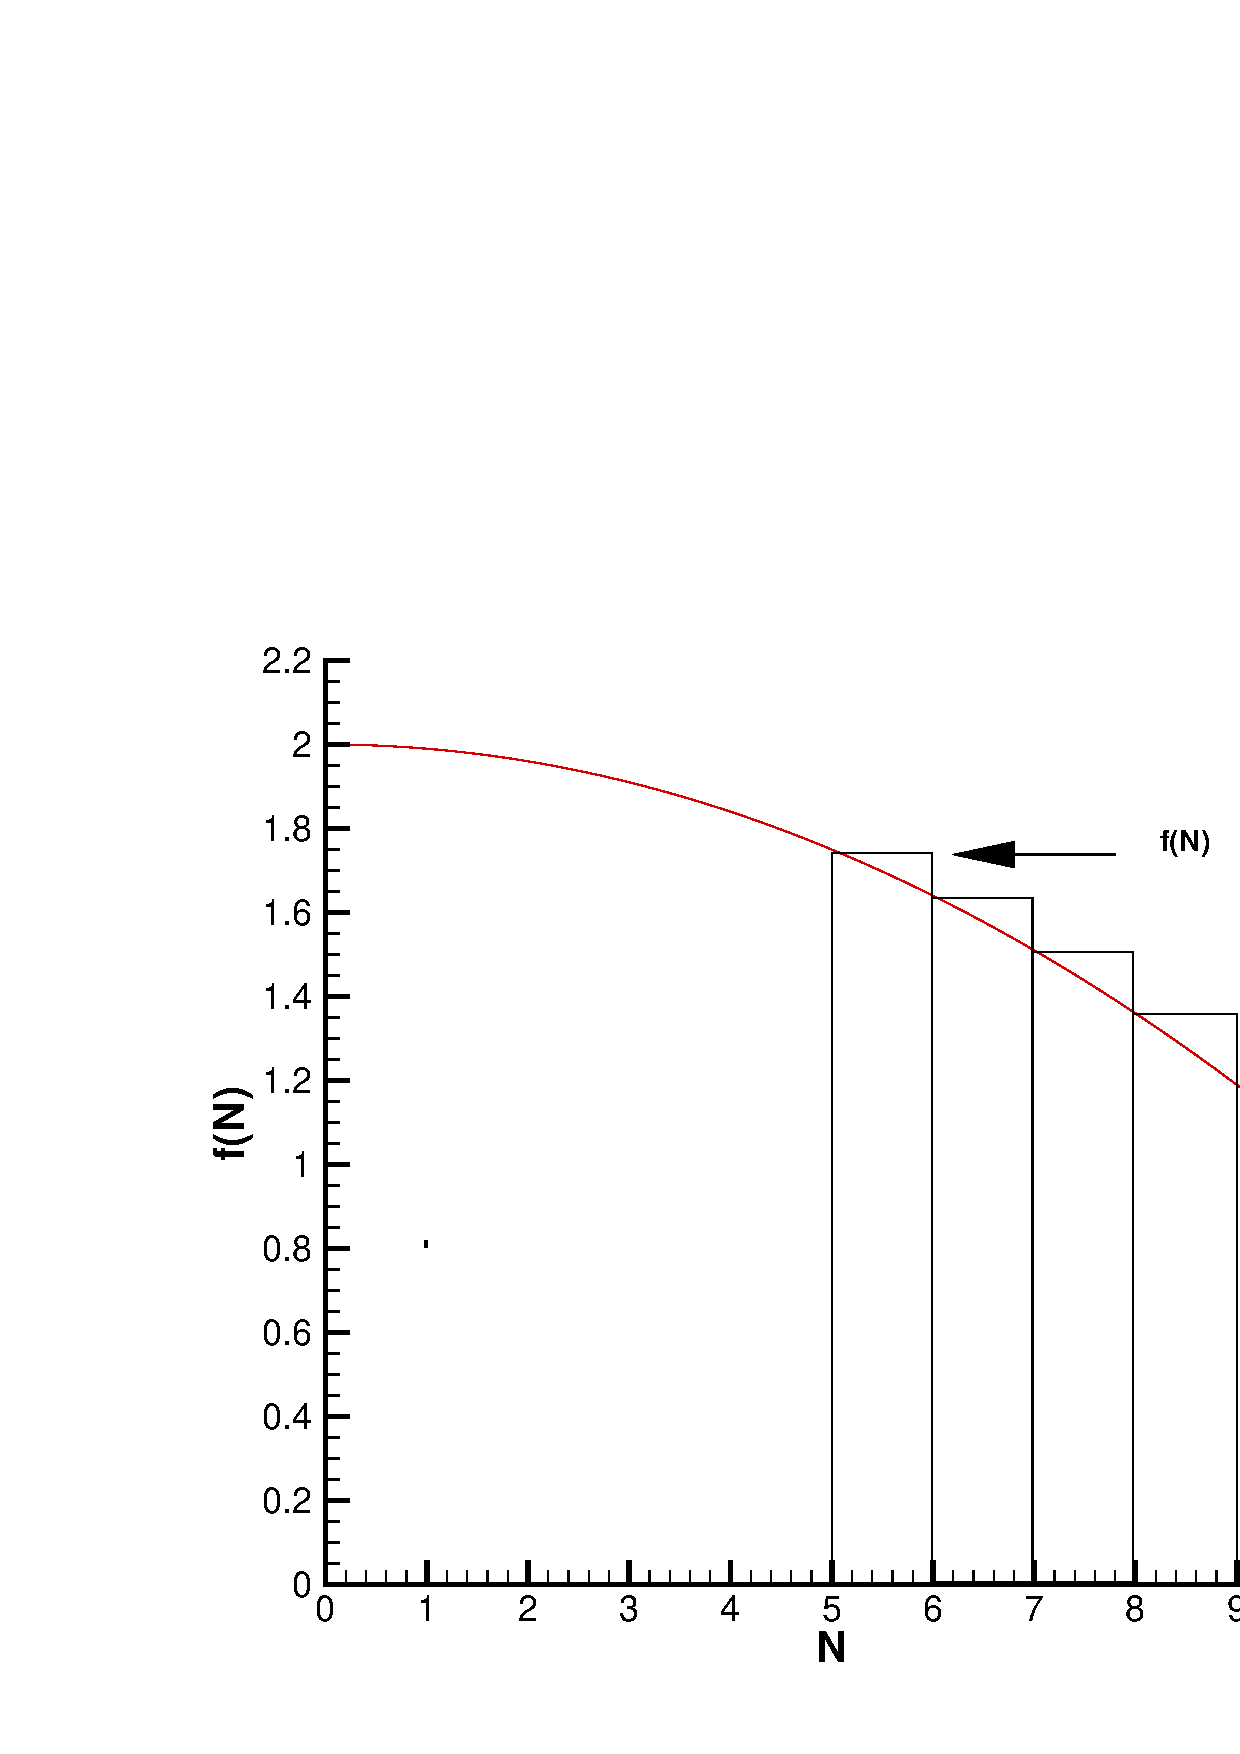
\includegraphics[width= 0.49\textwidth]{Figures/tecplot/sn.pdf}
	\caption{Relation between the integral of $ f:  \mathbb{R} \rightarrow \mathbb{R} $ and a sum of a numerical series with general term $ f 
	: \mathbb{N} \rightarrow \mathbb{R}$.}
	\label{fig:sn}
\end{figure}







    \FloatBarrier
    \subsection{Mathematical support for \texttt{Tail} function}
    
Notice that the function \texttt{Tail} is specially created for good convergence series. It is based on the premise that:
\begin{verbatim} 
    ! Obtain N such as:
    ! integral from i=N+1 to infinity a_i = eps
\end{verbatim}
For a fast convergence sum (the general term tends to 0 quickly), 
the sum is stopped when the truncation error is equal or less than some specific value \texttt{eps}. 
The terms not included in the sum would not appreciably
modify the result. 
For a sum series with a poor convergence the situation is the opposite, stopping the sum when the general term is less than \texttt{eps} 
leaves without adding a huge number of terms whose sum is comparable to \texttt{eps} or even much more higher. Then, the total error committed could be impermissible 
and there resides the difficulties of calculating these series.

Said in other words, the value \texttt{N} that \texttt{Tail} calculates is based on reducing the 
truncation error for good convergence series, not considering that it can be much higher than expected 
if round-off is reached before the truncation error is permissible.

    
    
    
    
    \subsection{First test for bad convergence sum}
For the example we are treating here the bounds of the error are:
\begin{equation}
    \frac{1}{N+1} \le \ S - S_N \ \le \frac{1}{N}
\end{equation} 
Being \texttt{S1} the result of the sum in the computer and using its analytical result,
the total error of the sum is $ \pi^2/6 - \texttt{S1} $.
Then, with the above bounds, the round-off error of the summation gives:

$$
    E_{fl} = E - E_N = \left( \frac{\pi^2}{6} - \texttt{S1} \right) - 1/N
$$
Let's execute now the following example to test this bad convergence sum series: 
\vspace{0.5cm}
\renewcommand{\home}{./Fortran/sources/Foundations/Calculus} 
\listings{\home/Examples/Sum_series.f90}{Summation_n2_examples}
{end subroutine}{Sum_Series.f90} 

First, take a look at the result of the computer if the summation process is stopped according to the 
round-off errors associated to significant digits. Notice that this result is obtained after 94906265 sums.

\begin{verbatim} 
Summation 1/n**2
S =  1.64493405783458   N =  94906265 Error = 9.013651380840315E-009
\end{verbatim}

Now force the computer to calculate the same sum up to 200000000 terms, 
around twice the number of operations than before,
notice that the total error is exactly the same than in the
previous case.

\begin{verbatim} 
S =  1.64493405783458   N = 200000000 Error = 9.013651380840315E-009
\end{verbatim}

If both errors are balanced thanks to the bounds calculated, 
the following results are obtained for the truncation and round-off errors 
(for \texttt{N = 94906265} terms added):

\begin{verbatim} 
Truncation error S =   1.053671197498475E-008
Round--off error   =  -1.523060594144434E-009
\end{verbatim}

Two interesting conclusions are obtained for this example. 
Firstly, 
the round-off error is quite smaller than the error associated to the truncation. 
Secondly,
the error is much higher than the finite number of digits that the computer 
is handling with the sums (in this case around 15 decimal digits). An infinite number of
non-negligible terms are omitted due to a bad convergence rate. 






    \subsection{Second test for bad convergence sum}

Now, the same sum is performed with declarative paradigm, 
calculate the result for a value \texttt{eps = 1e-10} 
and calculate the total error as usual:
\begin{verbatim} 
    real :: S, eps, E
    
    eps = 1e-10
    S = Sigma( a1, 1, eps )
    E = PI**2/6 - S
    
    write(*,*) " Summation 1/n**2 "
    write(*,*) " S = ", S, "Error = ", E    
\end{verbatim}

The following result is obtained, a total error of around \texttt{1e-5} is committed
when the computer is performing sums with terms around \texttt{1e-10}.  

\begin{verbatim} 
Summation 1/n**2
S =    1.64492406689824      Error =   9.999949984074163E-006
\end{verbatim}

A question may appear now; which \texttt{eps} should be introduced to \texttt{Sigma} so the result is calculated until round-off is obtained?
The answer is \texttt{eps = epsilon( S )/2.}, however, some notions of floating-point representation are essential to deepen in this topic.
An extensive discussion regarding the consistency of using \texttt{epsilon( S )} for this example and the generalization for any other sum 
is treated in the section \ref{chap:reals} of Part \ref{PartII} of this book. Also, why dividing it by \texttt{2} is needed becomes clearer. 




 
    \subsection{How can I improve this calculation?}
    
There is a different way of calculating this sum with better accuracy in the computer:
\begin{enumerate}
    \item Using higher precision for the variables, for example quadruple precision for the variables involved. 
    \item Change the algorithm to perform the sum. A non-intuitive way of calculating the sum comes from the fact
    that adding in floating-point arithmetic is not an associative operation. 
\end{enumerate}

Let's perform the same sum backwards, also with double precision and from the lower terms to the higher ones using 1000000000 terms, more than 10 times the maximum terms
used for the forward sum. 

\begin{verbatim} 
Summation 1/n**2
S = 1.64493406584823 N = 1000000000 Error = 1.000000082740371E-009

Truncation error S =   1.000000000000000E-009
Round --off error =   8.274037093680878E-017
\end{verbatim}
 
Surprisingly, just performing the same sums from the lower terms to the higher ones the 
limit of terms found before can be exceeded and the result is ten times more accurate than before. 
As a general rule, when adding numbers with a big difference in magnitude order, 
try to sum first the lower values and then add the result to the higher values. 
Why this improve the result is 
treated in the section \ref{chap:reals} of Part \ref{PartII} of this book.
 
 

\label{numeric_series}








%Dar el resultado de la suma de los 100 primeros términos de las siguientes series: 
%\begin{enumerate}    
%	\item Serie de números naturales.
%	\item Serie de números naturales impares.
%	\item Serie numérica donde el término general de la serie es: $ a_n = 1/n^2 $ desde $ n= 1 $.  
%	\item Serie numérica donde el término general de la serie es $ a_n = 1/ n! $ desde $ n=1$.  % e 
%	\item Serie numérica donde el término general de la serie es
%	$ a_n = (-1)^{n+1}/ (2n-1) $ desde $ n=1$.   
%\end{enumerate}         



%___________________________________________________________________________________________________
\newpage 
\section{Convergence rate}  \label{sec:convergence} 
One of the main focus of the numerical approximation techniques is to attain expansions with high rate of convergence. When dealing with 
numerical series, it is desirable to obtain a precise result by adding the smallest number ot terms to reduce CPU time. 
However, the number of terms to obtain the precise accuracy depends on the convergence rate of the series.
In other words, the behavior of $ a_n $ with $ n \rightarrow \infty $ defines the number of terms to be added. 



In figure \ref{spectral},  $ a_n $ versus $ n $ is represented in log-scale. 
In the same context of discretization techniques, 
if $ a_n = O( 1/n^q) $  for a  given number $ q $, the convergence is algebraic. 
If $ a_n \ll O( 1/n^q) $ for all  q, the convergence is spectral. 
This is shown schematically in figure \ref{spectral}.
\unitlength 0.8mm
\begin{center}
	\begin{figure}[htbp]
		\centering
		\vbox{
			\begin{picture}(120,85)
			
			%   \put(0,0){\framebox(120,85)}
			
			\drawline [200](40,70)(80,50)               
			\drawline [200](40,65)(80,35) 
			\drawline [200](40,60)(80,20)           
			
			\put(30,10){\vector(0,1){70}}
			\put(30,10){\vector(1,0){70}}   
			
			\put(10,78){$\log{|a_{n}|}$}                                        
			\put(90,5){$\log{n}$}
			\put(85,35){Algebraic (line with slope $ q $)}            
			
			\put(38,20){Spectral}    
			
			\qbezier(40,55)(55,40)(60,10)
			
			\qbezier(90,60)(90,40)(70,20)
			
			\put(70,20){\vector(-1,-1){0}}          
			
			
			
			\end{picture} 
			\caption{Convergence of $ a_n $ with $ n $.  Algebraic and spectral  convergence. }
			\label{spectral}
		}
		
	\end{figure}
\end{center}





 
 
 
 
 
   
   